% -*- root: ../../main.tex -*
%!TEX root = ../../main.tex
% vim:textwidth=80 fo=cqt conceallevel=0

\afterpage{\clearpage}

\begin{figure}[p]
    \begin{minipage}[t]{\textwidth}
        \centering
        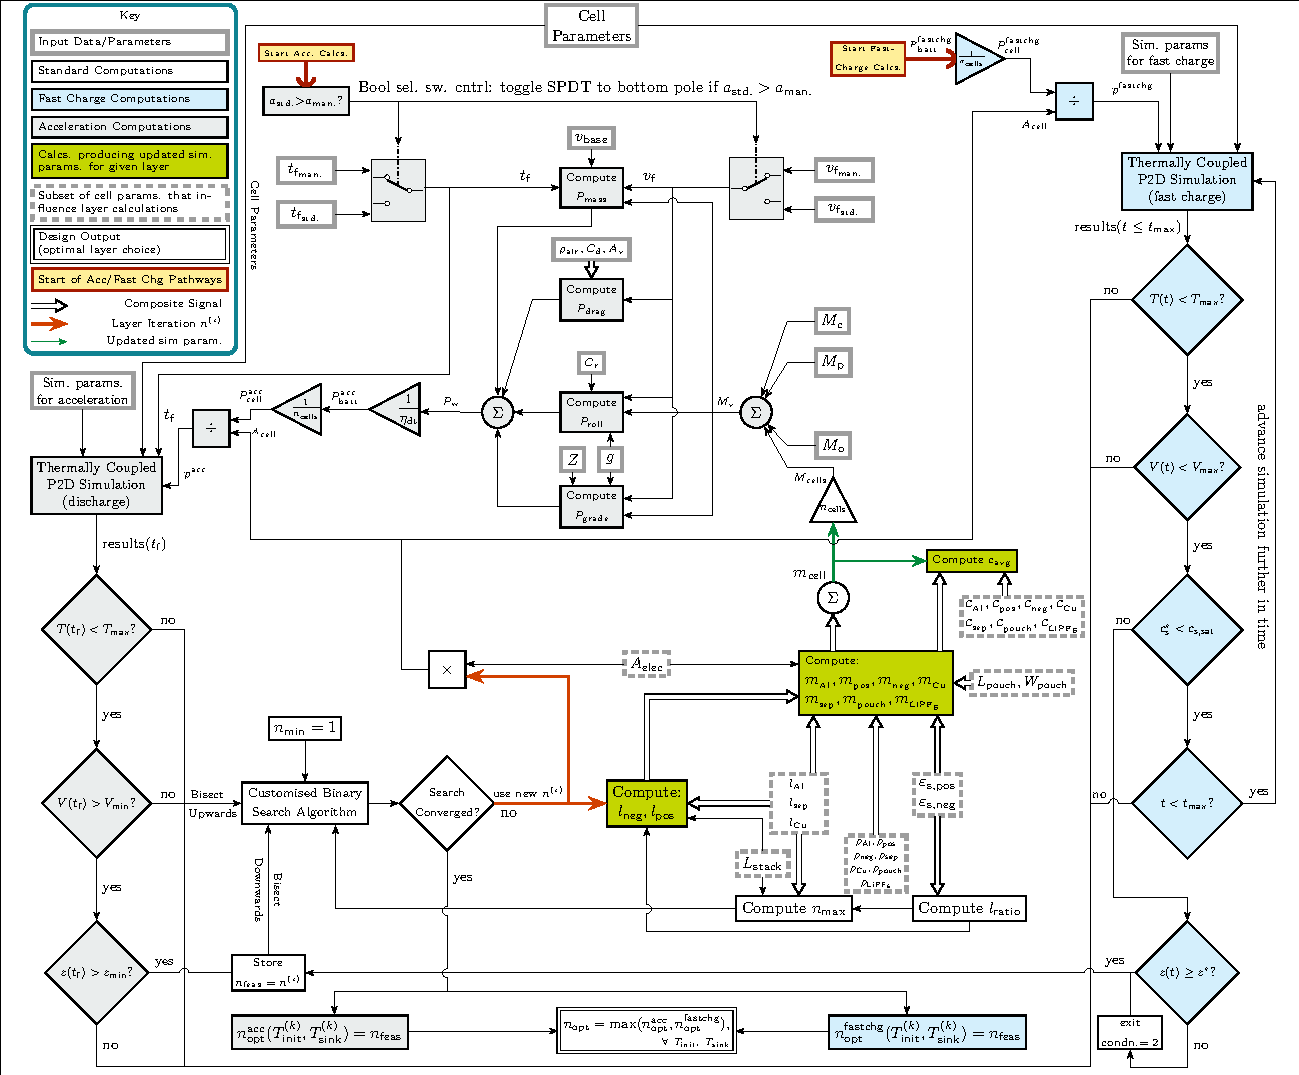
\includegraphics[angle=90, width=\textwidth]{fig_master_flow_diagram}
        \captionsetup{labelsep=note}
        \caption
        [%
        Flow diagram depicting an overview of the proposed layer optimisation methodology
        for Li-ion pouch cells.
        ]%
        {%
            Flow diagram depicting an overview of the proposed layer optimisation methodology
            for Li-ion pouch cells.
        }%
        \label{fig:fig_strategy_schematic}
        \mpfootnotes[1]
        % \vspace*{1.125cm}
        \vspace*{0.7225cm}
        \footnote{This figure was created by \mbox{Krishnakumar Gopalakrishnan} who
            asserts copyright, with intellectual contributions from and the right to
        use asserted by \mbox{Ian Campbell}.}
    \end{minipage}
\end{figure}

\subsection{Electrode thickness ratio for capacity balancing}

A key  idea of the layer  optimisation scheme is that  for computing the
physical  lengths  of electrode  as  a  function  of number  of  layers,
the  ratios  of  their thicknesses~$l_\text{ratio}$  is  held  constant.
This  coefficient is  germane to  the concept  of capacity  balancing of
electrodes  to equalise  their loading and is computed as follows.

Equating  the active material volume of both electrodes,
\begin{equation}
    A_\text{elec,pos}l_\text{pos}  \varepsilon_\text{s,pos} = A_\text{elec,neg}l_\text{neg}  \varepsilon_\text{s,neg} \label{eqn:electrodeCapacity}\\
\end{equation}

Neglecting  overhangs   of  the  negative  electrode   (typically  below
$\SI{2}{\milli\meter}$ to  avoid plating  at the edges),  both electrode
materials have the same cross-sectional area~$A_\text{elec}$. Therefore,
\cref{eqn:electrodeCapacity} reduces to
\begin{align}
    \cancel{A_\text{elec}}l_\text{pos}  \varepsilon_\text{s,pos} & = \cancel{A_\text{elec}}l_\text{neg}  \varepsilon_\text{s,neg}  \\
    l_\text{pos}  \varepsilon_\text{s,pos}                       & = l_\text{neg}  \varepsilon_\text{s,neg}\label{eqn:electrodeCapequalarea}
\end{align}

For the reference cell under consideration, the length and breadth of the cell's
pouch is  obtained from the \gls{bev}  manufacturer~\cite{GMBoltBatteryDims} and
are listed in \cref{tbl:lcoSimParamslayeropt}.

% % double-check if electrode area or overall area or what ?


% As  a  first-order  approximation  the
% product of  these dimensions can  be assumed  to be the  active material
% cross-sectional  area   (although  in  practice,  the   planar  area  of
% the  stack  needs to  be  slightly  smaller  to be  accommodated  inside
% the  pouch).  Finally,  in  line   with  the  assumptions  discussed  in
% \cref{subsec:layeroptassumptions},  similar  to  the pouch  height,  the
% cross-sectional geometry (length  and breadth) of the cell  is also held
% constant throughout the layer optimisation process.

Owing to the reasons  outlined in \cref{subsec:layeroptassumptions}, the
volume fractions of the electrode  materials are assumed to be constant,
which  implies  that their  ratio  is  also  a constant.  The  electrode
thickness ratio~$l_\text{ratio}$ is obtained as
\begin{alignat}{2}
    l_\text{ratio} & = \frac{l_\text{neg}}{l_\text{pos}}                                                                                  &  & \qquad\text{(by definition)}                                          \\
    {}             & = \frac{\varepsilon_\text{s,pos}}{\varepsilon_\text{s,neg}}                                                          &  & \qquad\text{(rearranging \cref{eqn:electrodeCapequalarea})}           \\
    {}             & = \frac{1-\varepsilon_\text{pos} - \varepsilon_\text{fi,pos}}{1-\varepsilon_\text{neg} - \varepsilon_\text{fi,neg}}  &  & \qquad\text{(by definition)}                                          \\
    {}             & = \frac{1- 0.385 - 0.025}{1 - 0.485 - 0.033}                                                                         &  & \qquad\text{(substituting values from \cref{tbl:lcoSimParamsSPMp2d})} \\
    l_\text{ratio} & = 1.22\label{eqn:electrodeThicknessRatio}
\end{alignat}

% Do not forget to quote the value of cs_sat from layer opt paper table and show
% calculation inline. Might even go into the code
